\documentclass[12pt,a4paper]{article}
\usepackage[italian]{babel}
\usepackage[T1]{fontenc}
\usepackage[latin1]{inputenc}
\usepackage{graphicx}
\usepackage{amsmath}
\usepackage{subfig}
\date{}
\begin{document}
\title{Strutture Aeronautiche\\ Esercitazione 3 \\ Prof.re Franco Mastroddi}
\author{Matteo Hakimi 1455230}
\maketitle
\begin{figure}[htbp]
\centering

\includegraphics[width=100mm]{Immagini/1}
\end{figure}
\newpage
\tableofcontents
\newpage


\section{Introduzione}
Si vogliono calcolare i modi propri ed il campo di spostamento (in due diverse condizioni di carico), di una piastra in alluminio rettangolare di lati a=4 m e b=5 m di spessore t=3 mm appoggiata sui 4 lati.
Il calcolo verr\'a svolto tramite l'uso di solutore agli elementi finiti, utilizzando 2 discretizzazioni della struttura.
Infine si effettuer\'a il confronto della soluzione con quella ottenuta per via analitica.
\begin{figure}[htbp]
	\centering
	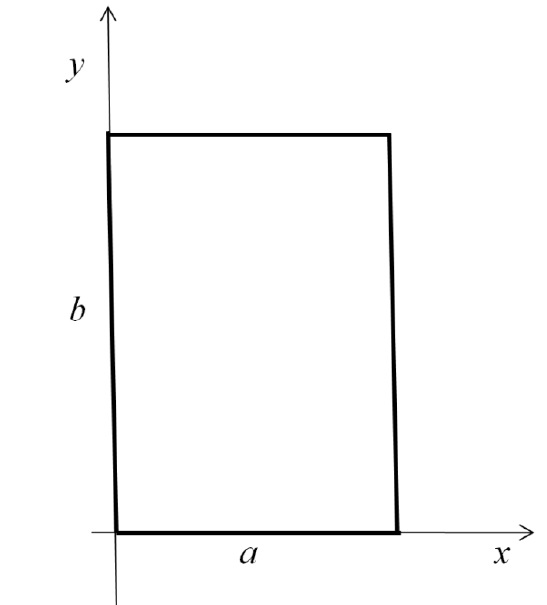
\includegraphics[scale=0.4]{Immagini/piastra.jpg}
	\caption{Piastra appoggiata}
\end{figure}
\section{Pressione uniforme}
Il primo caso analizzato � quello di un carico di pressione uniformemente distribuito sulla superficie della piastra stessa, di intensit� $P=200 N/m^{2}$ .\
Avendo ipotizzato la struttura assimilabile come una piastra puramente flessibile, dalla teoria analitica basata sull'approccio "alla Galerkin" scengliendo le funzioni di forma coincidenti con le autofunzioni (metodo delle autofunzioni) si ha che lo spostamento in direzione verticale rispetto al piano contenente la piastra � dato da: 
\begin{equation}
w(x,y)=\dfrac{16P}{D \pi^{2}}\sum_{m,n=1,3,5,...}^{\infty}\dfrac{\sin(\dfrac{m \pi x}{a})\sin(\dfrac{n \pi y}{b})}{mn[(\dfrac{m \pi}{a})^{2}+(\dfrac{n \pi}{b})^{2}]^{2}}
\end{equation}
dove D rappresenta la rigidezza flessionale della piastra.\\
Si riportano in tabella il valore dello spostamento al centro della piastra in funzione dei valori m,n di troncamento della serie.\\ \\
	\begin{tabular}{c c c}
		\hline
		 m & n& w [m]\\
		\hline
       1 &        1 & -1.830475 \\ 
       1 &        3 & -1.794563 \\ 
       1 &        5 & -1.797970 \\ 
       1 &        7 & -1.797299 \\ 
       3 &        1 & -1.779639 \\ 
       3 &        3 & -1.782150 \\ 
       3 &        5 & -1.781625 \\ 
       3 &        7 & -1.781769 \\ 
		\hline
	\end{tabular} \quad
		\begin{tabular}{c c c}
			\hline
			m & n& w [m]\\
			\hline
       5 &        1 & -1.783267 \\ 
       5 &        3 & -1.782920 \\ 
       5 &        5 & -1.783037 \\ 
       5 &        7 & -1.782993 \\ 
       7 &        1 & -1.782707 \\ 
       7 &        3 & -1.782786 \\ 
       7 &        5 & -1.782752 \\ 
       7 &        7 & -1.782768 \\ 
			\hline
		\end{tabular}\\ \\

Si pu\'o osservare che la serie converge abbastanza velocemente, si noti infatti che il termine ottenuto troncando la sommatoria a m=n=3 differisce di circa $10^{-4} m$ rispetto a quello successivo.\\ Possiamo quindi assumere (per i nostri scopi), che troncando la serie a m=n=3 si abbia una buona stima della soluzione.\\
Si � calcolata inoltre la risposta statica (SOL 101) della struttura utilizzando un codice agli elementi finiti,dopo aver opportunamente discretizzato la struttura prima con 10 e 16 elementi (non 15 perch� in seguito si vorr\'a mettere un carico concentrato nel nodo centrale al fine di valutarne lo spostamento ) (SHELL) rispettivamente lungo i lati a e b e poi con 20 e 30 elementi lungo i medesimi lati.\\
Lo spostamento massimo si ha in corrispondenza del nodo centrale.\\ \\
Caso mesh 10x16
\begin{center}
	\begin{tabular}{c c c c c c c}
		\hline
		      POINT ID.& T1&             T2&             T3&             R1&             R2&             R3\\
		                 94      &      0.0&            0.0&           -1.793269E+00&   1.533773E-13&  -1.170397E-10&   0.0\\
		      \hline
		      
		\hline
	\end{tabular}
\end{center}
Caso mesh 20x30
\begin{center}
	\begin{tabular}{c c c c c c c}
		\hline
		POINT ID.& T1&             T2&             T3&             R1&             R2&             R3\\
		\hline
		          326      &      0.0 &           0.0&           -1.786304E+00&   1.478681E-07&  -3.190725E-12&   0.0\\
		\hline
	\end{tabular}
\end{center} 
Si nota che le componenti sul piano (x,y) dello spostamento sono nulle in accordo con la teoria analitica.\\
La rotazione massima attorno a y si ottiene nei punti (0,2.5) (4,2.5) di stessa intensit\'a (1.453 rad) ma di verso opposto mentre quella attorno a x nei punti (2,0) (2,5) (1.216 rad), ovvero si ottiene a met\'a dei lati su cui la piastra ha il vincolo di appoggio, come era possibile prevedere anche dalla simmetria del problema.\\
Si riportano in figura le diverse soluzioni ottenute (analitica e FEM).
 
\begin{figure}[htbp]
\centering
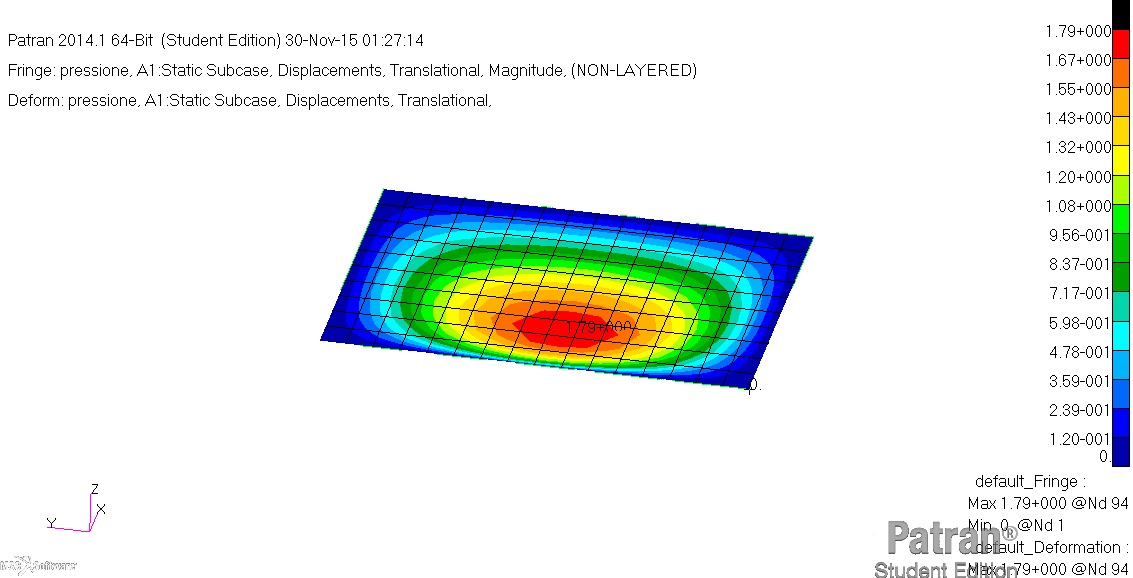
\includegraphics[scale=0.4]{Immagini/pressione.jpg}
\caption{Pressione uniforme, 10x16 elementi}
\end{figure}
\begin{figure}[htbp]
\centering
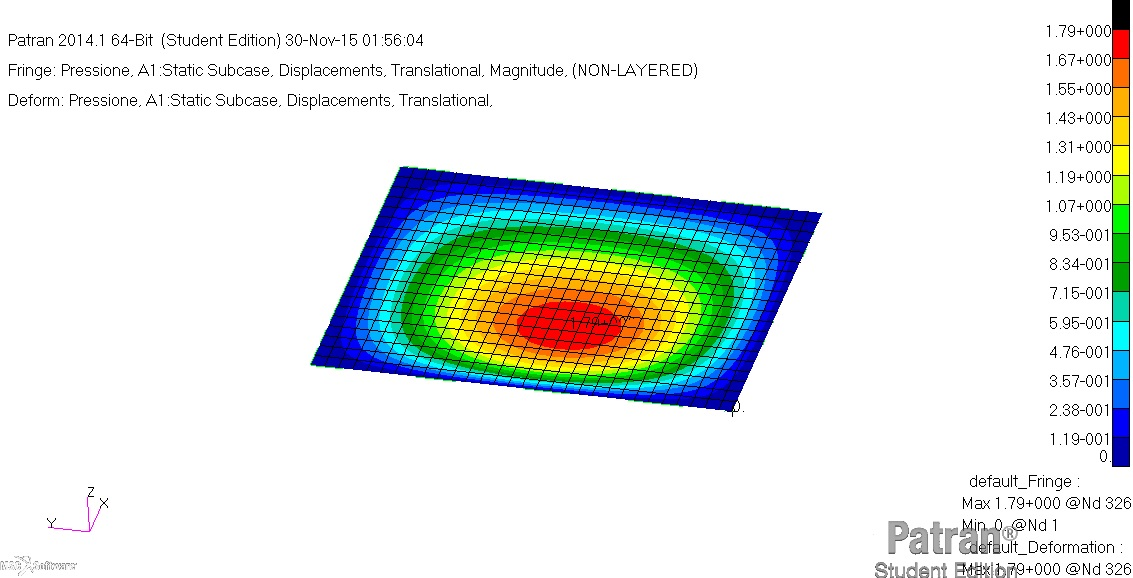
\includegraphics[scale=0.4]{Immagini/pressionefitta.jpg}
\caption{Pressione uniforme, 20x30 elementi}
\end{figure}
\begin{figure}[htbp]
	\centering
	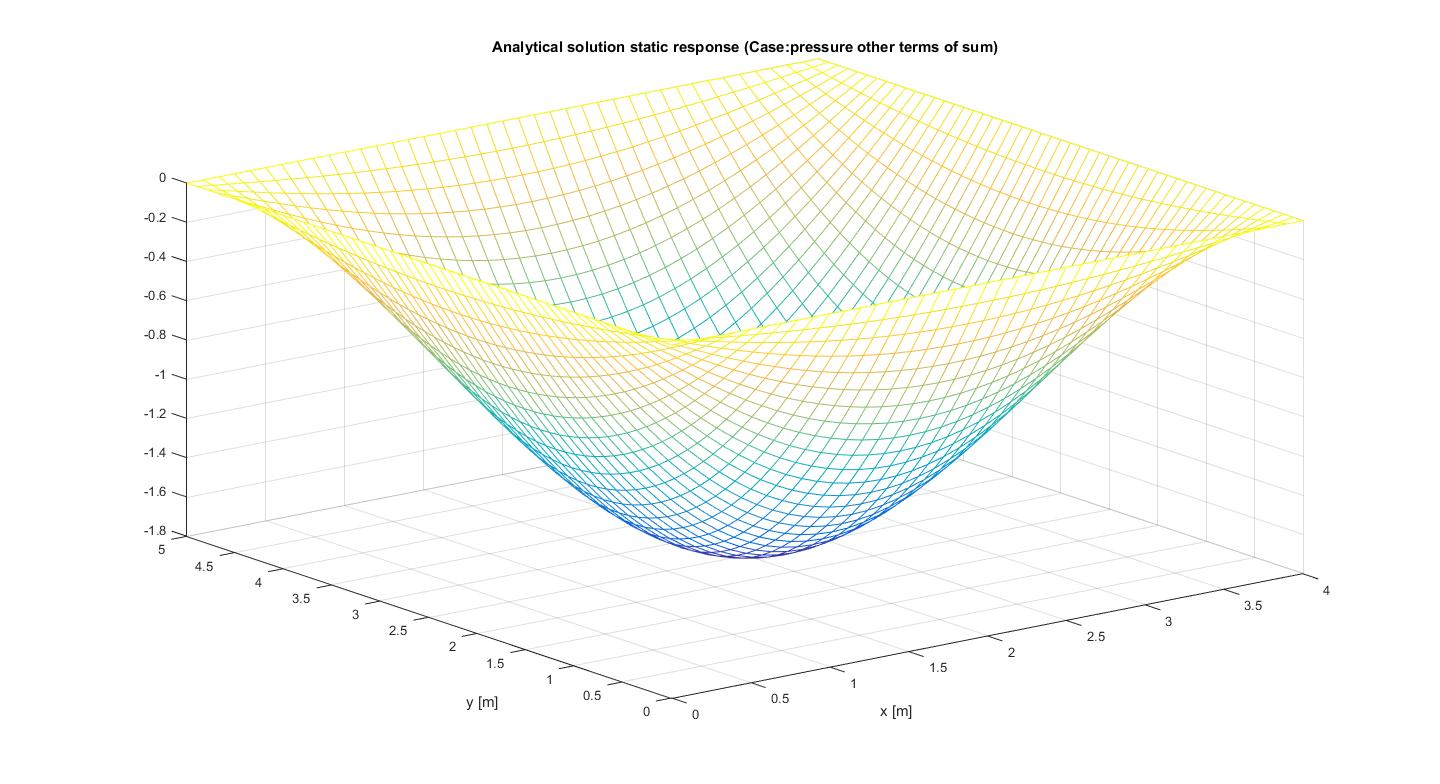
\includegraphics[scale=0.28]{Immagini/pressionemn.jpg}
	\caption{Pressione uniforme, analitica m=n=3}
\end{figure}
\newpage
Si osserva un andamento della soluzione ottenuta mediante solutore FEM in buon accordo con quello fornito dalla teoria;presentando uno spostamento massimo (in modulo) in corrispondenza del centro e un valore nullo ai bordi.\\
Si nota inoltre come l'andamento delle linee a spostamento costante (concentriche data la simmetria del problema) , differisce molto poco tra le diverse soluzioni.\\
Infine si riportano i valori di spostamento del punto centrale:
\begin{center}
	\begin{tabular}{c c}
		\hline
		w [m] & Soluzione \\
		\hline
			-1.830475 & Analitica m=n=1\\
				-1.782150 & Analitica m=n=3\\ 
				-1.793269E+00 &  FEM mesh 10x16 \\
		-1.786304E+00 & FEM mesh 20x30 \\
	\hline
	\end{tabular}
\end{center}

Si noti come infittendo la mesh si passa da un errore globale di $\epsilon=1.11\% $ ad un errore globale di $\epsilon=0.42\%$ l'errore � sceso dell $0.7\%$.\\
Tuttavia occorre precisare, che dato l'ordine di grandezza della soluzione $o(10^{1} m)$ rispetto a quello dello spessore $o(10^{3} m)$, l'ipotesi di piastra puramente flessibile non � pi� vera; ovvero l'intensit� del carico non rientra nel range di applicabilit� per gli stati di deformazione compatibili forniti dalla teoria di Kirchhoff, dove si ipotizza una deformazione dell'ordine dello spessore.  

\newpage


\section{Carico concentrato}
Nel secondo caso si � sostituito il carico distribuito con un carico equivalente concentrato al centro della piastra $F = 4000 N$.\\
Analogamente a quanto visto per il caso di pressione uniformente distribuita, si � assunto il modello di piastra puramente flessibile, e in accordo con la teoria analitica si ha:
\begin{equation}
w(x,y)=\dfrac{4F}{D S}\sum_{m,n=1,3,5,...}^{\infty}\dfrac{\sin(\dfrac{m \pi x}{a})\sin(\dfrac{m \pi }{2})\sin(\dfrac{n \pi y}{b})\sin(\dfrac{n \pi}{2})}{[(\dfrac{m \pi}{a})^{2}+(\dfrac{n \pi}{b})^{2}]^{2}}
\end{equation}
Dove S � la superficie della piastra, S=ab.\\
Si riportano in tabella il valore dello spostamento al centro della piastra in funzione dei valori m,n di troncamento della serie.\\ \\ \\ \\ \\ \\
	\begin{tabular}{c c c}
		\hline
		m & n& w [m]\\
		\hline
		       1 &        1 & -4.516516 \\ 
		       1 &        3 & -4.782343 \\ 
		       1 &        5 & -4.824376 \\ 
		       1 &        7 & -4.835976 \\ 
		       1 &        9 & -4.840327 \\ 
		       1 &       11 & -4.842302 \\ 
		       1 &       13 & -4.843321 \\ 
		       1 &       15 & -4.843899 \\ 
		       3 &        1 & -4.974617 \\ 
		       3 &        3 & -5.030377 \\ 
		       3 &        5 & -5.049813 \\ 
		       3 &        7 & -5.057270 \\ 
		       3 &        9 & -5.060552 \\ 
		       3 &       11 & -5.062178 \\ 
		       3 &       13 & -5.063063 \\ 
		       3 &       15 & -5.063582 \\ 
		\hline
	\end{tabular} \quad
		\begin{tabular}{c c c}
			\hline
			m & n& w [m]\\
			\hline
			5 &        1 & -5.082060 \\ 
			5 &        3 & -5.094899 \\ 
			5 &        5 & -5.102125 \\ 
			5 &        7 & -5.105949 \\ 
			5 &        9 & -5.108007 \\ 
			5 &       11 & -5.109164 \\ 
			5 &       13 & -5.109849 \\ 
			5 &       15 & -5.110275 \\ 
			7 &        1 & -5.115204 \\ 
			7 &        3 & -5.119255 \\ 
			7 &        5 & -5.122131 \\ 
			7 &        7 & -5.124012 \\ 
		    7 &        9 & -5.125206 \\ 
			7 &       11 & -5.125966 \\ 
			7 &       13 & -5.126458 \\ 
			7 &       15 & -5.126784 \\ 
			
			\hline
		\end{tabular} \quad
		\begin{tabular}{c c c}
			\hline
			m & n& w [m]\\
			\hline
		
			9 &        1 & -5.128607 \\ 
			9 &        3 & -5.130220 \\ 
			9 &        5 & -5.131512 \\ 
			9 &        7 & -5.132474 \\ 
			9 &        9 & -5.133162 \\ 
			9 &       11 & -5.133646 \\ 
			9 &       13 & -5.133986 \\ 
			9 &       15 & -5.134226 \\ 
			11 &        1 & -5.135046 \\ 
			11 &        3 & -5.135803 \\ 
			11 &        5 & -5.136450 \\ 
			11 &        7 & -5.136973 \\ 
			11 &        9 & -5.137380 \\ 
			11 &       11 & -5.137688 \\ 
			11 &       13 & -5.137919 \\ 
			11 &       15 & -5.138092 \\ 
			\hline
		\end{tabular} \quad
			\begin{tabular}{c c c}
				\hline
				m & n& w [m]\\
				\hline
				13 &        1 & -5.138515 \\ 
				13 &        3 & -5.138912 \\ 
				13 &        5 & -5.139267 \\ 
				13 &        7 & -5.139570 \\ 
				13 &        9 & -5.139819 \\ 
				13 &       11 & -5.140019 \\ 
				13 &       13 & -5.140177 \\ 
				13 &       15 & -5.140301 \\ 
				15 &        1 & -5.140540 \\ 
				15 &        3 & -5.140768 \\ 
				15 &        5 & -5.140977 \\ 
				15 &        7 & -5.141162 \\ 
				15 &        9 & -5.141320 \\ 
				15 &       11 & -5.141453 \\ 
				15 &       13 & -5.141563 \\ 
				15 &       15 & -5.141652 \\ 
				\hline
			\end{tabular}
		\newpage
Si pu\'o osservare che la serie questa volta converge pi� lentamente rispetto al caso precedentemente trattato, si noti infatti che il termine ottenuto troncando la sommatoria a m=n=3 differisce di circa $10^{-2}m$ rispetto a quello successivo, stabilizzandosi per m=15 n=7.\\ La necessit� di aggiungere pi\'u armoniche alla sommatoria per migliorare la soluzione nell'intorno del punto dove � applicato il carico \'� dovuta alla natura singolare del carico concentrato stesso in termini spaziali.\\
Si � calcolata inoltre la risposta statica (SOL 101) della struttura utilizzando un codice agli elementi finiti,dopo aver opportunamente discretizzato la struttura prima con 10 e 16 elementi (poich� si vuole mettere il carico nel punto centrale) (SHELL) rispettivamente lungo i lati a e b e poi con 20 e 30 elementi lungo i medesimi lati.\\
Lo spostamento massimo si ha in corrispondenza del nodo centrale.\\ \\
Caso mesh 10x16
\begin{center}
	\begin{tabular}{c c c c c c c}
		\hline
		POINT ID.& T1&             T2&             T3&             R1&             R2&             R3\\
           94      &      0.0 &           0.0 &          -5.233809E+00&   3.899901E-13&   8.056322E-09&   0.0\\
		\hline
		
		\hline
	\end{tabular}
\end{center}
Caso mesh 20x30
\begin{center}
	\begin{tabular}{c c c c c c c}
		\hline
		POINT ID.& T1&             T2&             T3&             R1&             R2&             R3\\
		\hline
		           326      &      0.0  &          0.0&           -5.181973E+00&   2.022009E-07&  -8.568539E-10&   0.0\\
		\hline
	\end{tabular}
\end{center}
In accordo a quanto visto nel caso precedente lo spostamento sul piano risulta nullo e i punti di massima rotazione coincidono con quelli precedenti in particolare si ha che la rotazione massima lungo x � 2.455 rad quella lungo y 3.418 rad.\\
Si riportano in figura le diverse soluzioni ottenute (analitica e FEM).

\begin{figure}[htbp]
\centering
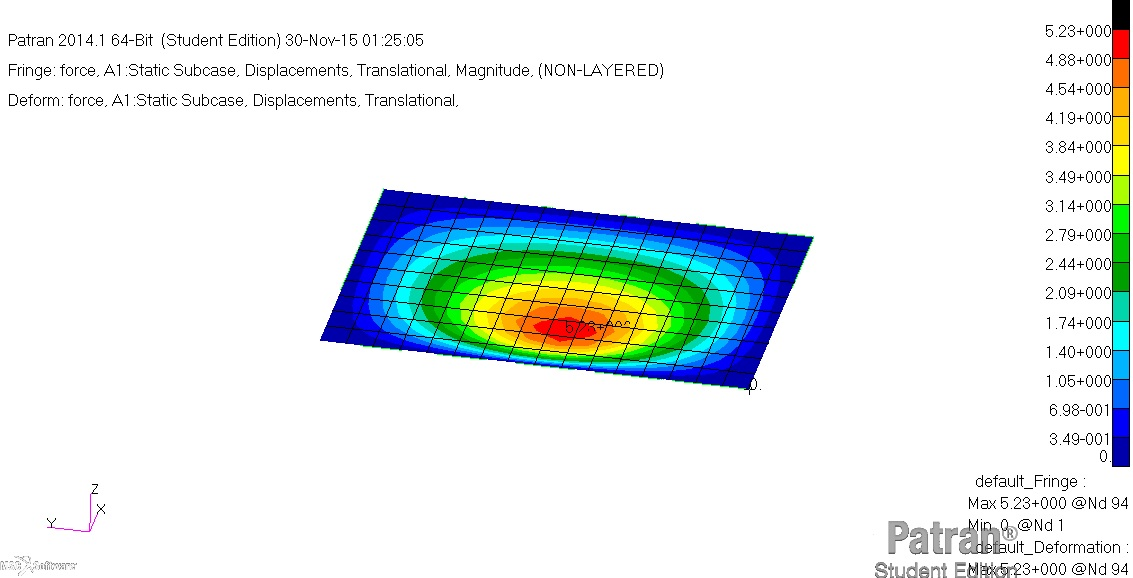
\includegraphics[scale=0.4]{Immagini/forza.jpg}
\caption{Carico concentrato, 10x15 elementi}
\end{figure}

\begin{figure}[htbp]
\centering
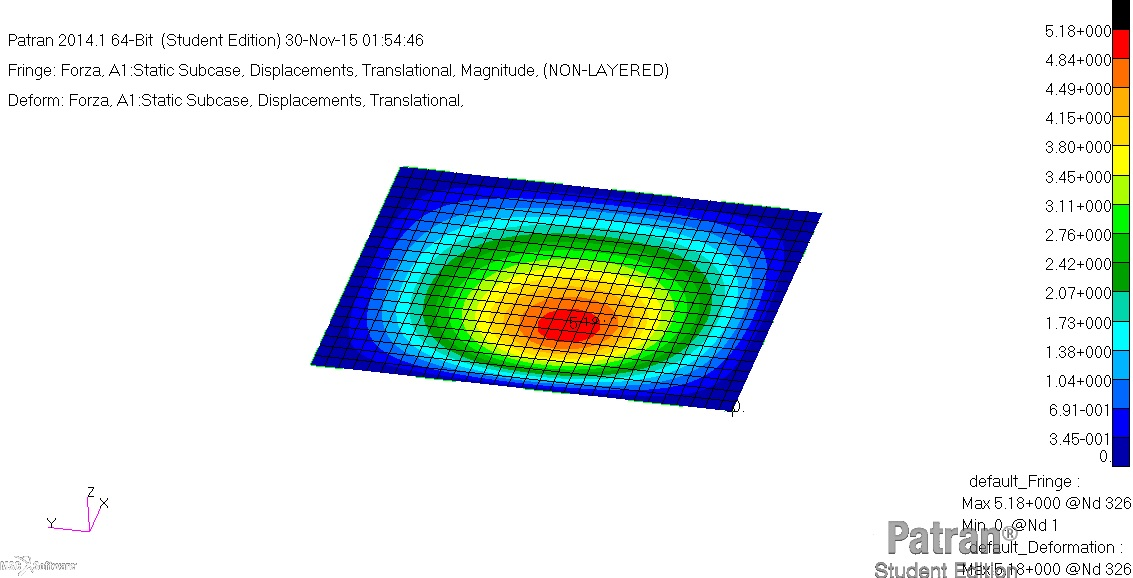
\includegraphics[scale=0.4]{Immagini/forzafitta.jpg}
\caption{Carico concentrato, 20x30 elementi}
\end{figure}

\begin{figure}[htbp]
	\centering
	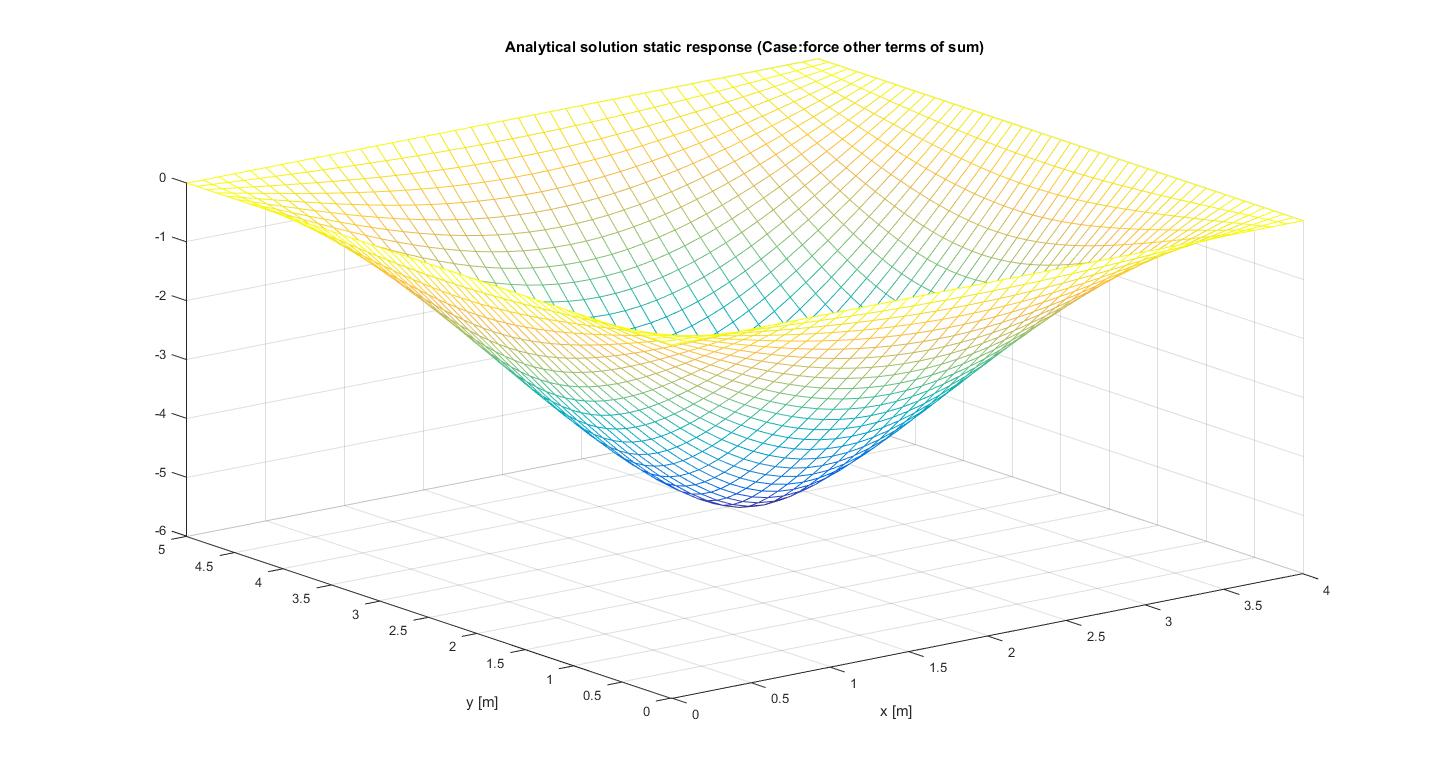
\includegraphics[scale=0.28]{Immagini/forzamn}
	\caption{Carico concentrato, analitica m=n=15}
\end{figure}
\newpage
Anche in questo caso l'andamento della soluzione ottenuta con codice FEM risulta in buon accordo con quella ottenuta analiticamente.\\
Infine si riportano i valori di spostamento del punto centrale:
\begin{center}
	\begin{tabular}{c c}
		\hline
		w [m] & Soluzione \\
		\hline
		-4.516516  & Analitica m=n=1\\
		-5.141652 & Analitica m=n=15\\ 
		-5.233809E+00&  FEM mesh 10x16 \\
		 -5.181973E+00 & FEM mesh 20x30 \\
		\hline
	\end{tabular}
\end{center}

Si noti come infittendo la mesh si passa da un errore globale di $\epsilon=9.22\% $ ad un errore globale di $\epsilon=4.02\%$ rispetto al caso precedente l'errore � sceso, a parit\'a di infittimento, del $5.20\%$, si nota invece che l'errore commesso che si ha troncando la soluzione a m=n=1 e quella a m=n=15 � di $\epsilon=62.51\%$\\ 
Tuttavia occorre precisare, ancora una volta che che dato l'ordine di grandezza della soluzione $o(10^{1} m)$ rispetto a quello dello spessore $o(10^{3} m)$, l'ipotesi di piastra puramente flessibile non � pi� vera.  
\newpage


\section{Modi Propri}
Il terzo ed ultimo caso prevede il calcolo dei primi 12 modi di vibrare; quest'ultimi, e le rispettive pulsazioni, sono state calcolati mediante il codice FEM (SOL 103), avendo discretizzato la struttura con 20 e 30 elementi lungo i lati a e b rispettivamente, e normalizzando tali modi rispetto al massimo  dello spostamento (MAX) in modo da ottenere una rappresentazione  con valore massimo pari a 1.\\Infine viene riportata la loro rappresentazione prevista dalla teoria analitica in cui ricordiamo  che il generico modo �:
\begin{equation}
\varphi_{mn}(x,y)=C\sin(\dfrac{m \pi x}{a})\sin(\dfrac{n \pi y}{b})
\end{equation}
Dove $C=\dfrac{2}{\sqrt{ab}}$.\\
Si riportano in tabella i valori delle pulsazioni ottenute tramine Nastran e quelle ricavate analiticamente.
Ricordiamo che:
\begin{equation}
\omega_{mn}^{2}=\dfrac{D}{\rho t}[(\dfrac{m \pi}{a})^{2}+(\dfrac{n \pi}{b})^{2}]^{2} 
\end{equation}
\begin{center}
	\begin{tabular}{c c c c c}
		\hline
		Modo & n & m & $\omega_{mn}$ Analitica [rad/s] & $\omega$ FEM [rad/s] \\
\hline
1 &        1 &        1 & 4.592018 & 4.581230 \\ 
2 &        1 &        2 & 9.968038 & 9.926906 \\ 
3 &        2 &        1 & 12.992050 & 12.950650 \\ 
4 &        2 &        2 & 18.368071 & 18.209100 \\ 
5 &        1 &        3 & 18.928073 & 18.840260 \\ 
6 &        3 &        1 & 26.992104 & 26.906030 \\ 
7 &        2 &        3 & 27.328105 & 26.987730 \\ 
8 &        1 &        4 & 31.472121 & 31.324720 \\ 
9 &        3 &        2 & 32.368125 & 32.035540 \\ 
10 &        2 &        4 & 39.872153 & 39.299420 \\ 
11 &        3 &        3 & 41.328159 & 40.606980 \\ 
12 &        4 &        1 & 46.592179 & 46.454400 \\ 
\hline
\end{tabular}
\end{center}
Si nota un buon accordo tra le frequenze proprie di vibrazione calcolate con il codice agli elementi finiti e quelle esatte.
Infine vengono riportati le prime 12 deformate corrispondenti.
\newpage
\begin{figure}
	\subfloat[][\emph{Modo 1 FEM}.]
	{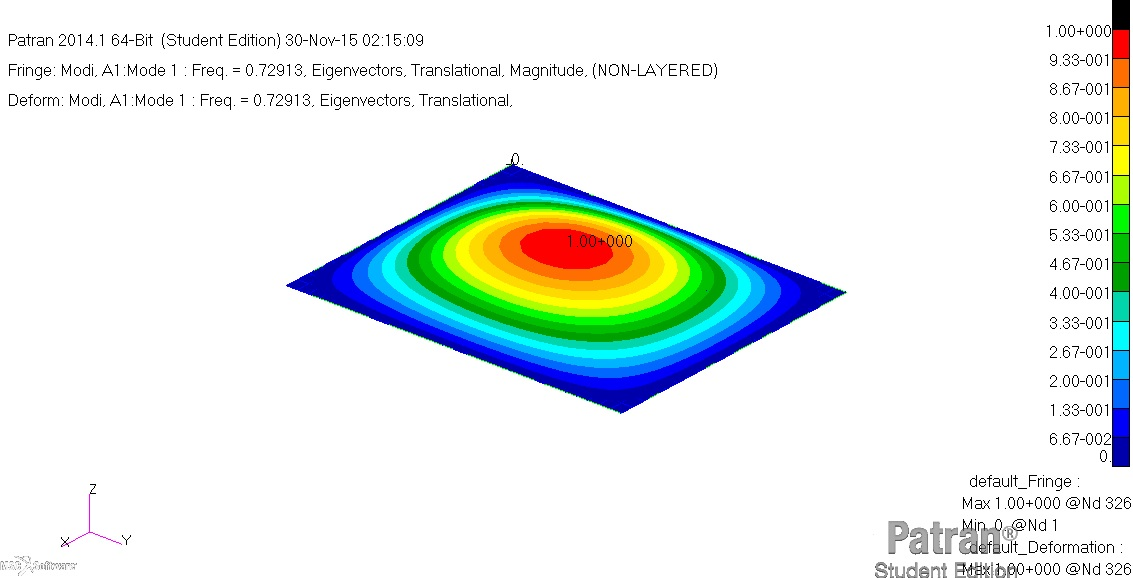
\includegraphics[width=.55\textwidth]{Immagini/modo1p.jpg}} \quad
	\subfloat[][\emph{Modo 1 Analitico}.]
	{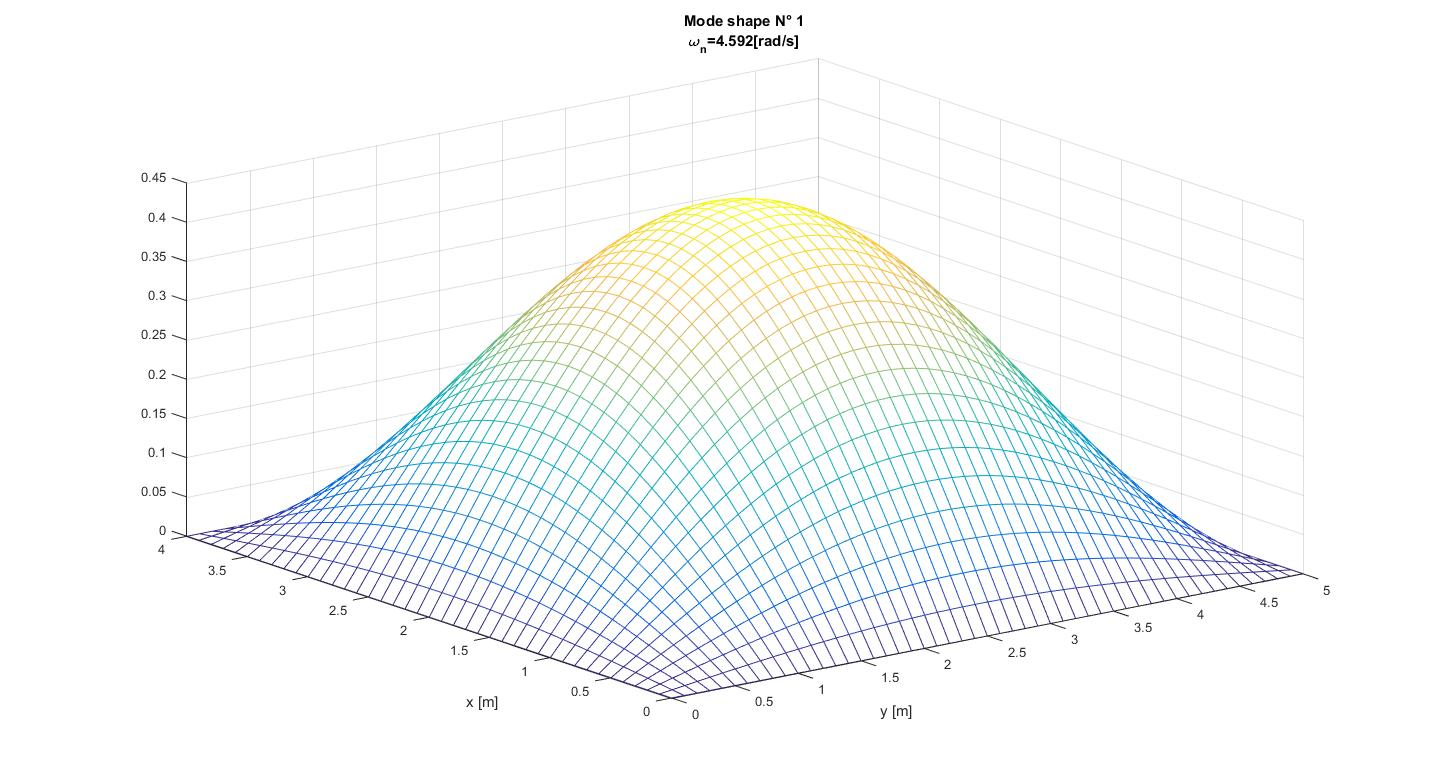
\includegraphics[width=.55\textwidth]{Immagini/modo1.jpg}} 
	\label{fig:subfig}
\end{figure}
\begin{figure}
	\subfloat[][\emph{Modo 2 FEM}.]
	{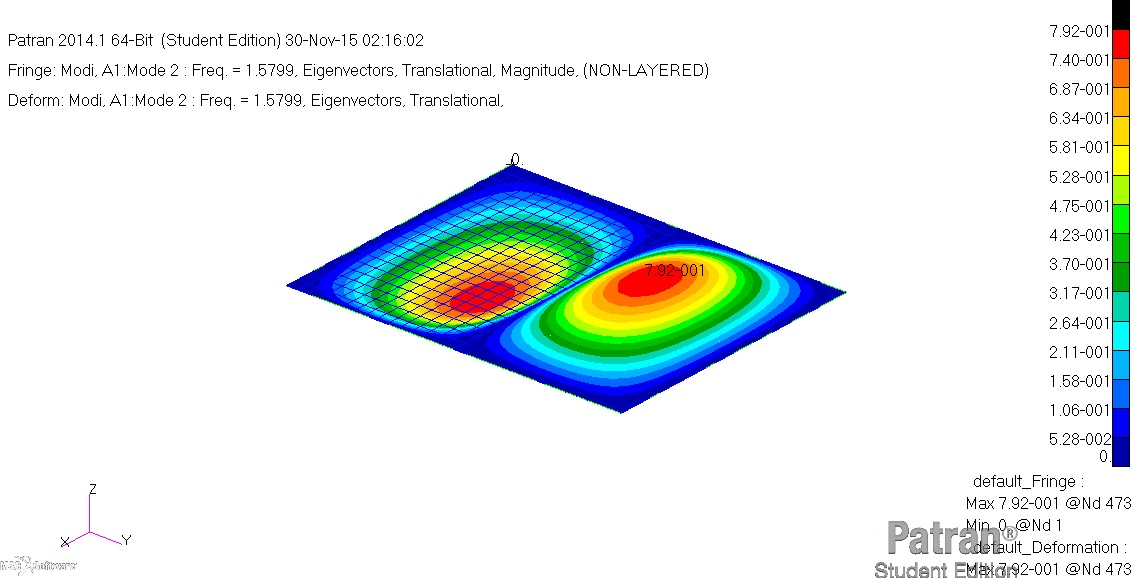
\includegraphics[width=.55\textwidth]{Immagini/modo2p.jpg}} \quad
	\subfloat[][\emph{Modo 2 Analitico}.]
	{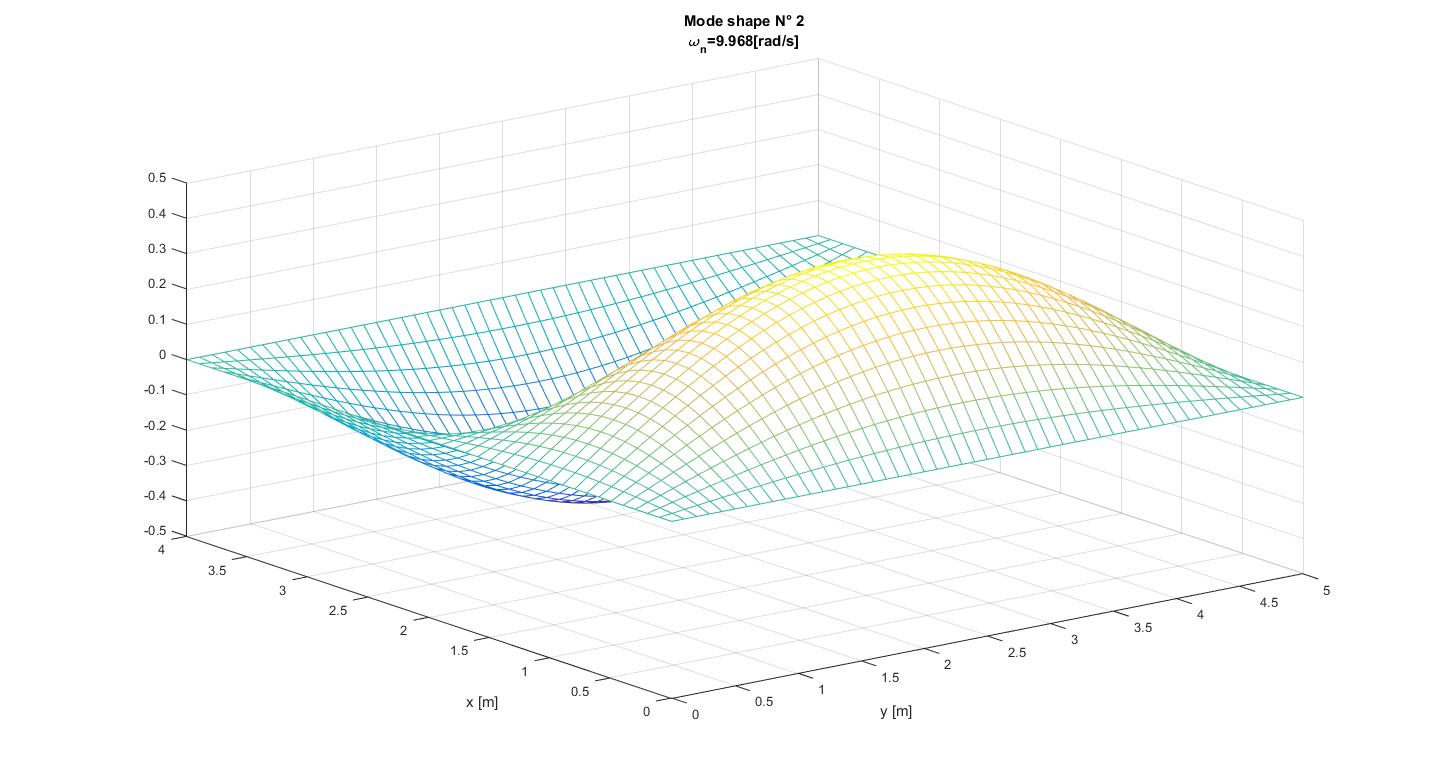
\includegraphics[width=.55\textwidth]{Immagini/modo2.jpg}} 
	\label{fig:subfig}
\end{figure}
\begin{figure}
	\subfloat[][\emph{Modo 3 FEM}.]
	{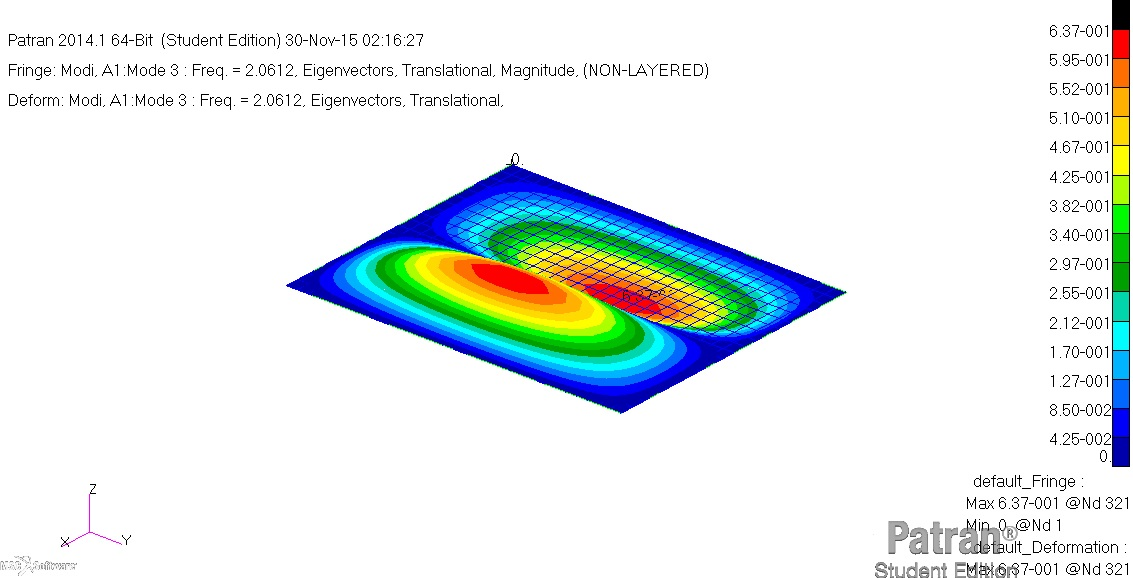
\includegraphics[width=.55\textwidth]{Immagini/modo3p.jpg}} \quad
	\subfloat[][\emph{Modo 3 Analitico}.]
	{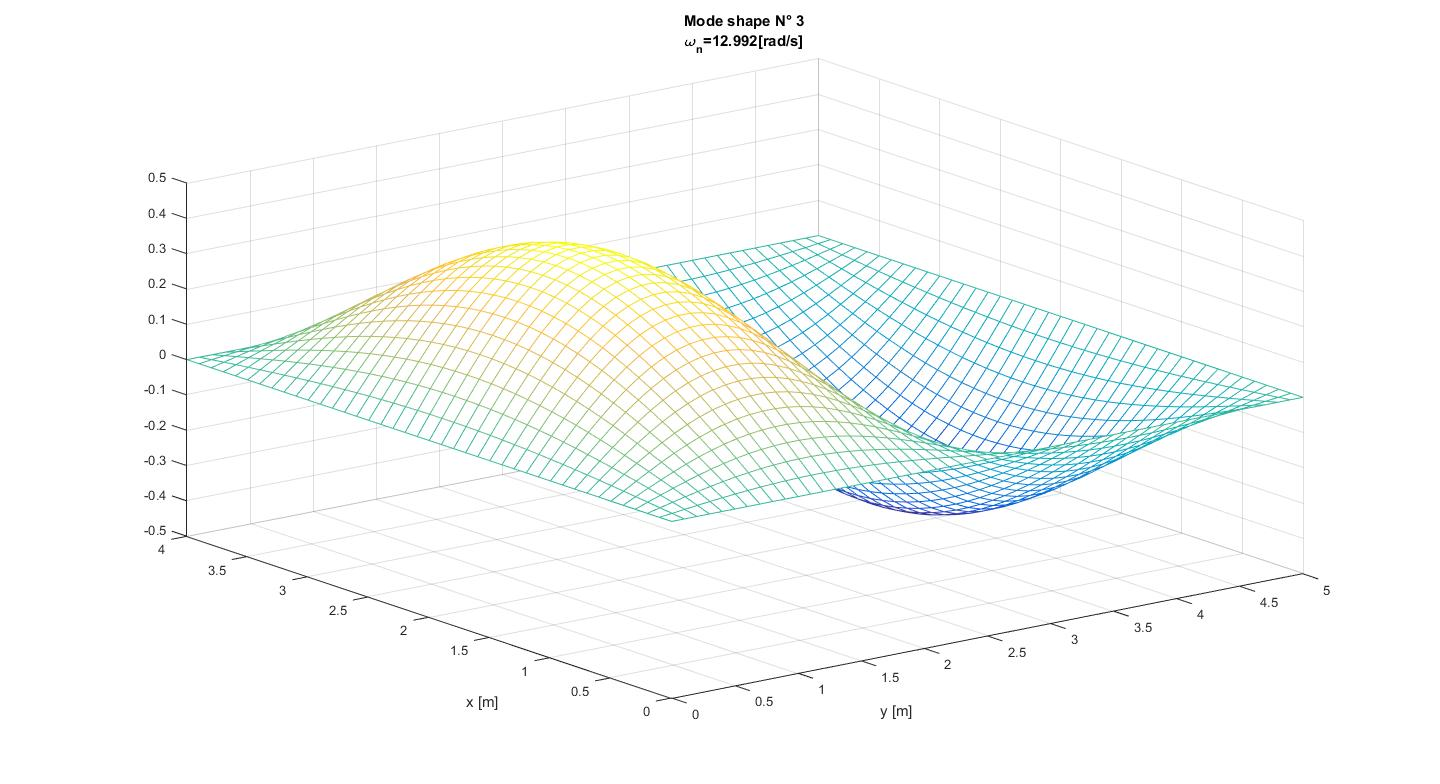
\includegraphics[width=.55\textwidth]{Immagini/modo3.jpg}} 
	\label{fig:subfig}
\end{figure}
\begin{figure}
	\subfloat[][\emph{Modo 4 FEM}.]
	{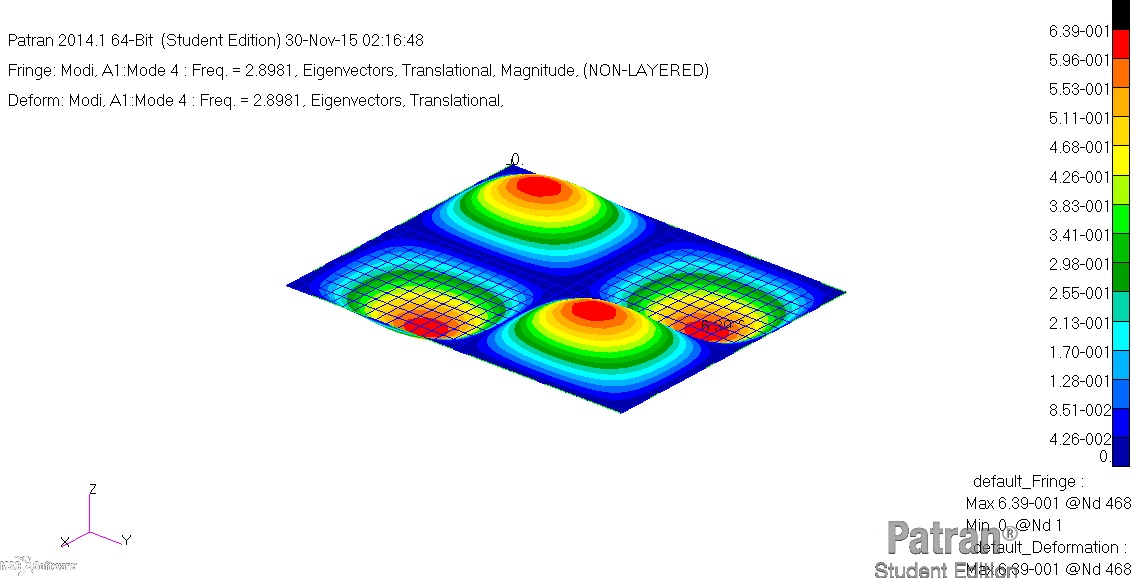
\includegraphics[width=.55\textwidth]{Immagini/modo4p.jpg}} \quad
	\subfloat[][\emph{Modo 4 Analitico}.]
	{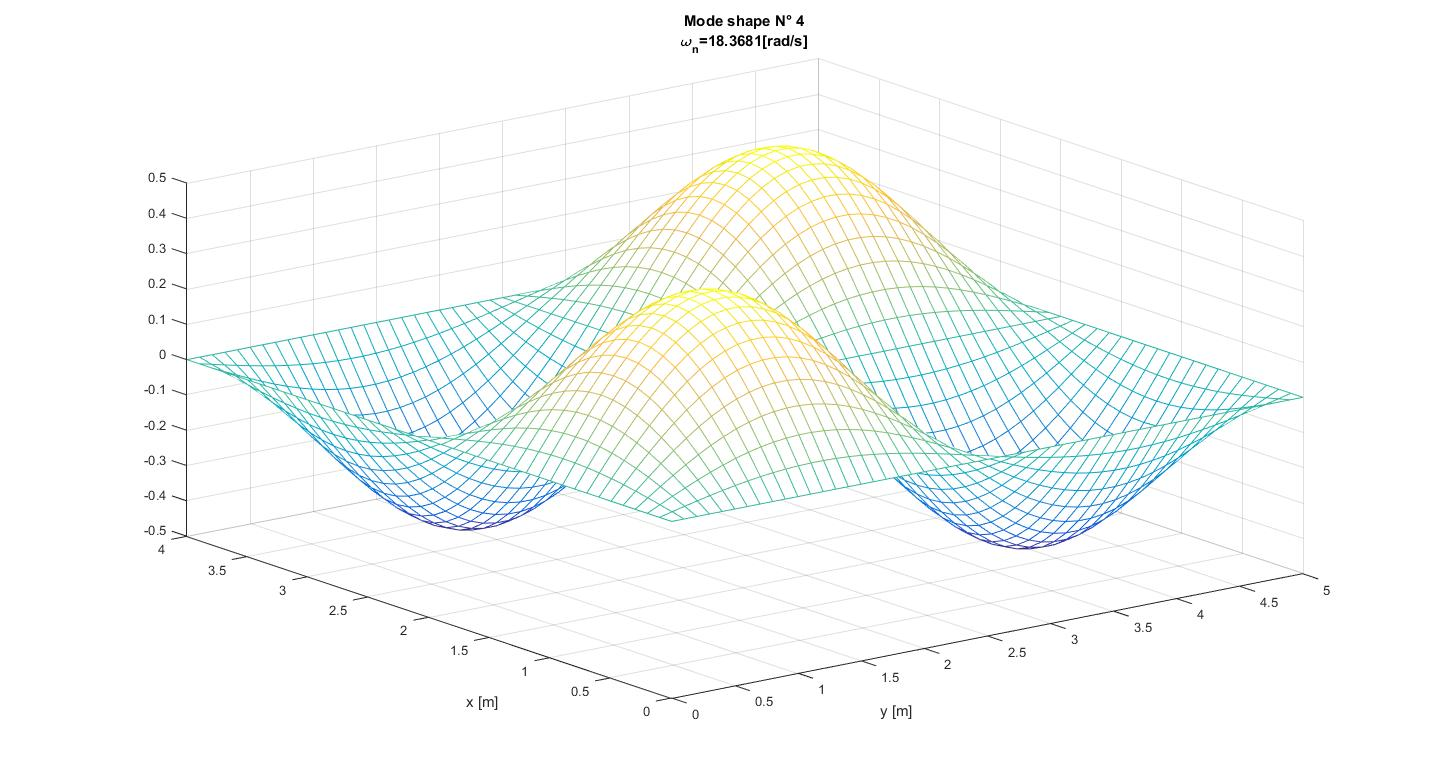
\includegraphics[width=.55\textwidth]{Immagini/modo4.jpg}} 
	\label{fig:subfig}
\end{figure}

\begin{figure}
	\subfloat[][\emph{Modo 5 FEM}.]
	{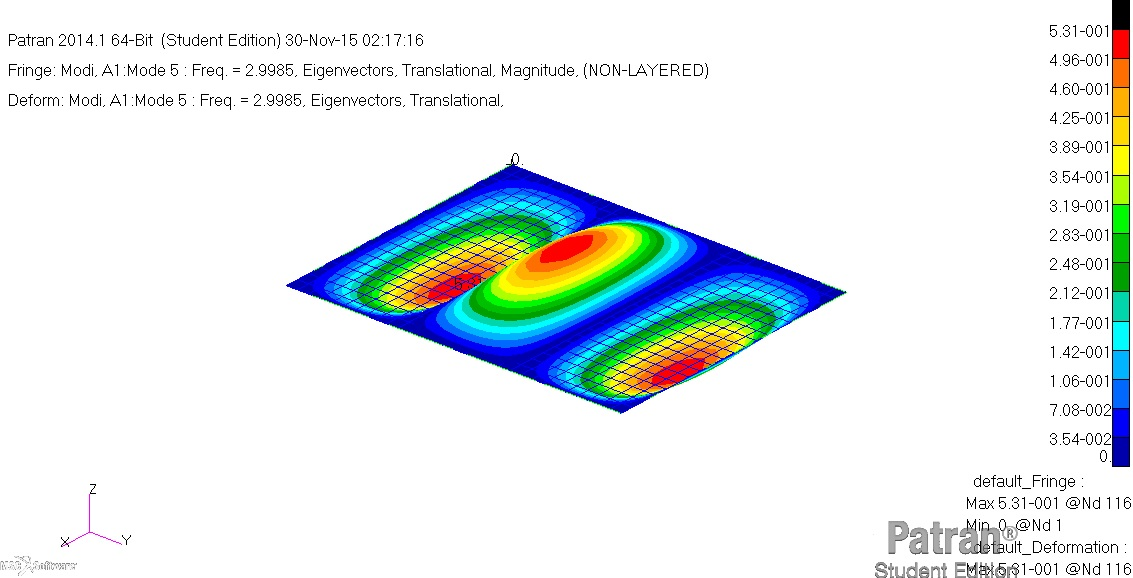
\includegraphics[width=.55\textwidth]{Immagini/modo5p.jpg}} \quad
	\subfloat[][\emph{Modo 5 Analitico}.]
	{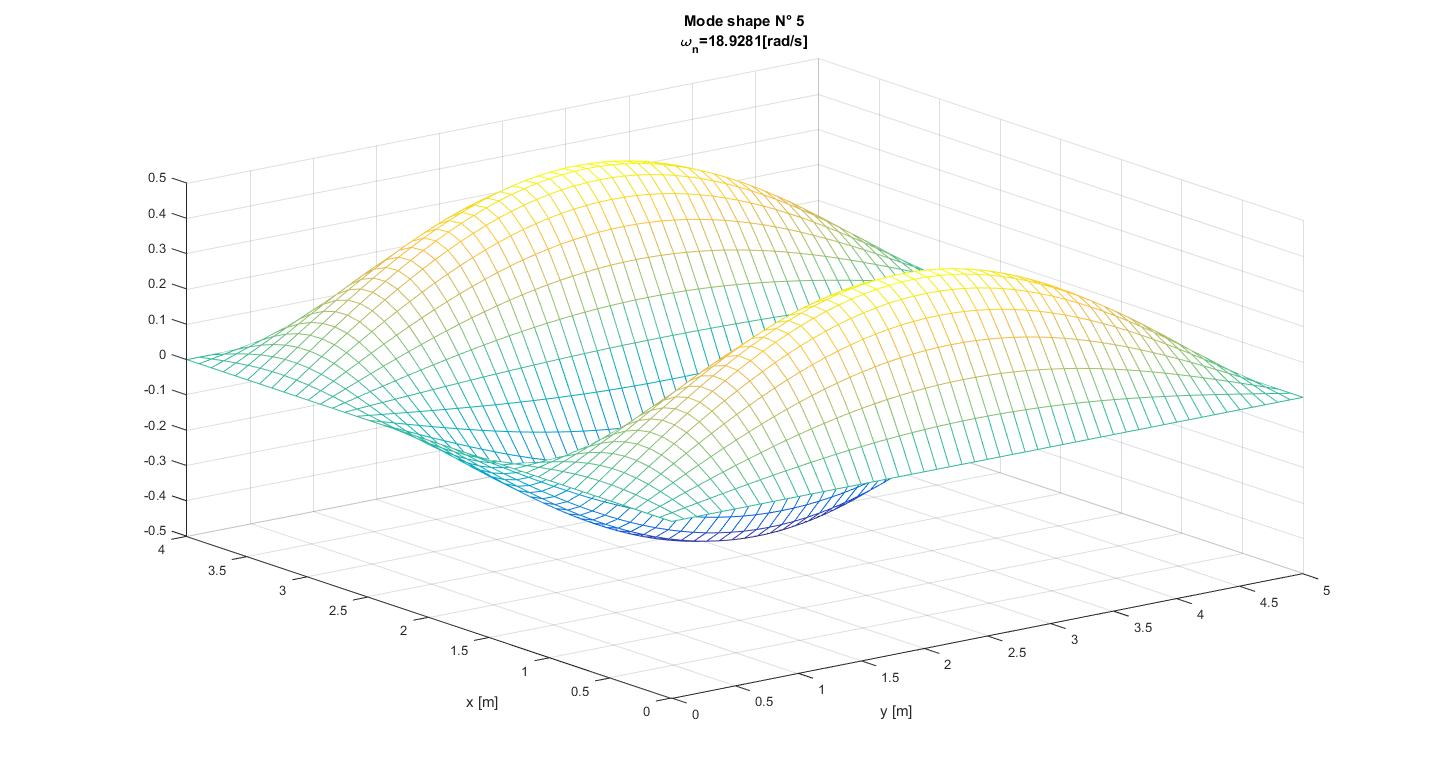
\includegraphics[width=.55\textwidth]{Immagini/modo5.jpg}} 
	\label{fig:subfig}
\end{figure}

\begin{figure}
	\subfloat[][\emph{Modo 6 FEM}.]
	{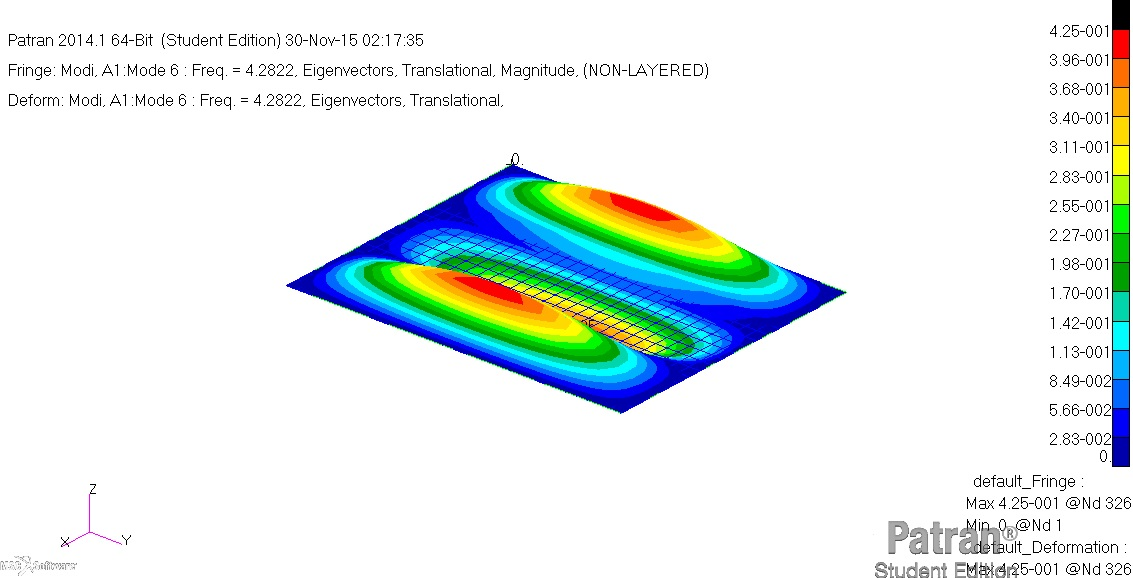
\includegraphics[width=.55\textwidth]{Immagini/modo6p.jpg}} \quad
	\subfloat[][\emph{Modo 6 Analitico}.]
	{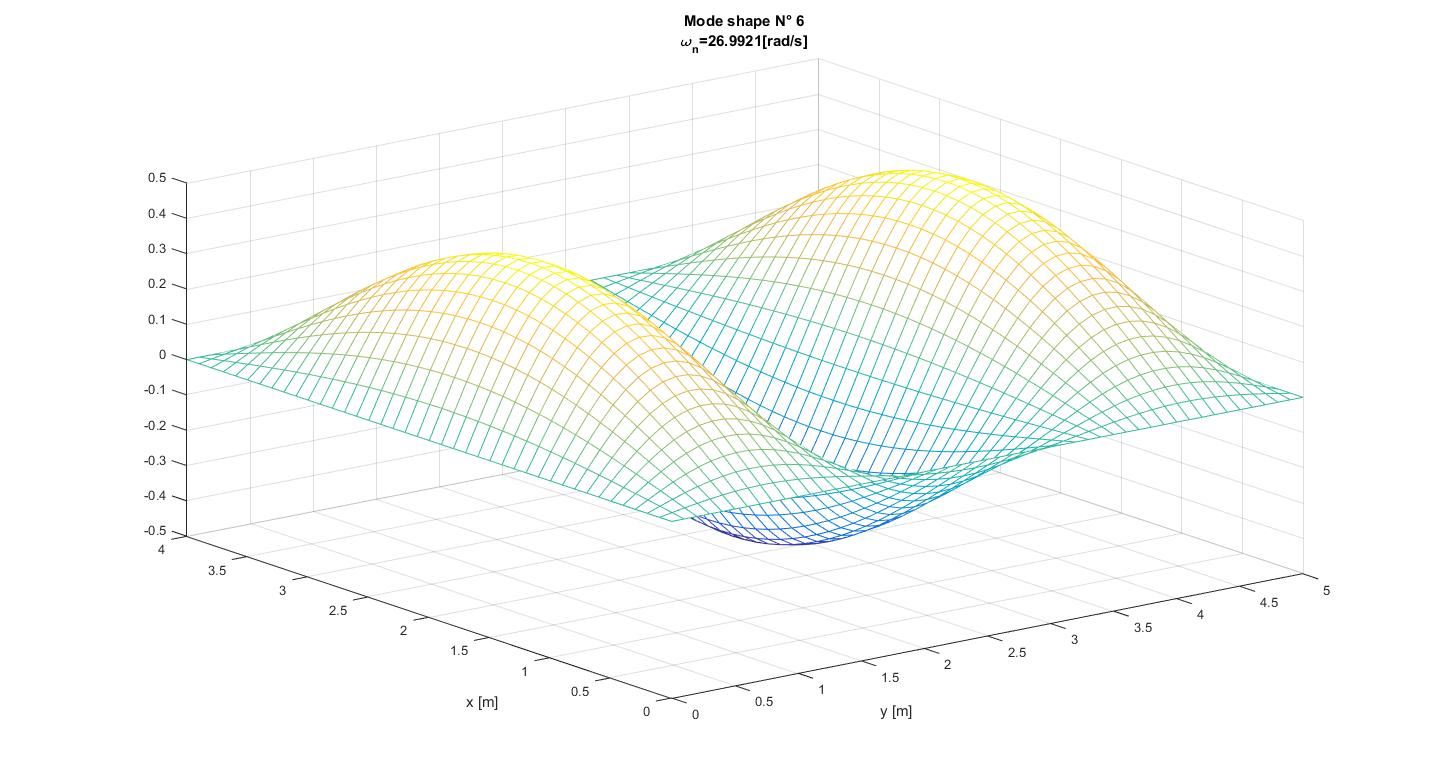
\includegraphics[width=.55\textwidth]{Immagini/modo6.jpg}} 
	\label{fig:subfig}
\end{figure}

\begin{figure}
	\subfloat[][\emph{Modo 7 FEM}.]
	{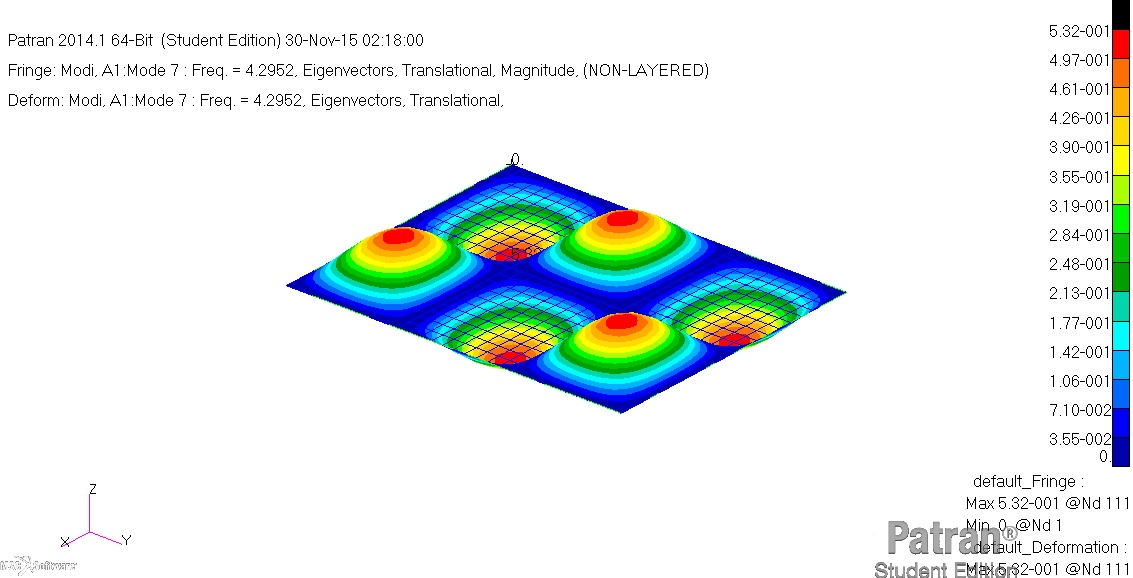
\includegraphics[width=.55\textwidth]{Immagini/modo7p.jpg}} \quad
	\subfloat[][\emph{Modo 7 Analitico}.]
	{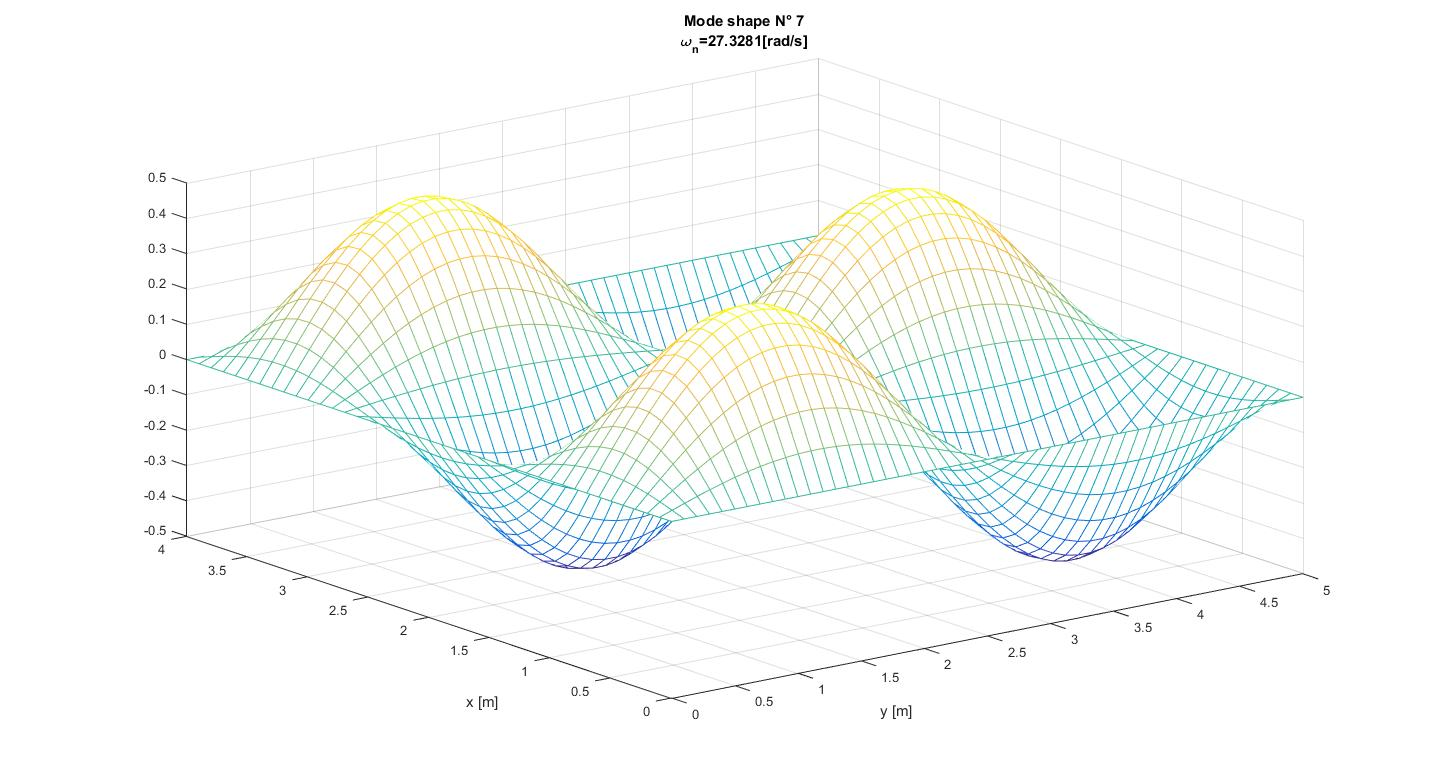
\includegraphics[width=.55\textwidth]{Immagini/modo7.jpg}} 
	\label{fig:subfig}
\end{figure}

\begin{figure}
	\subfloat[][\emph{Modo 8 FEM}.]
	{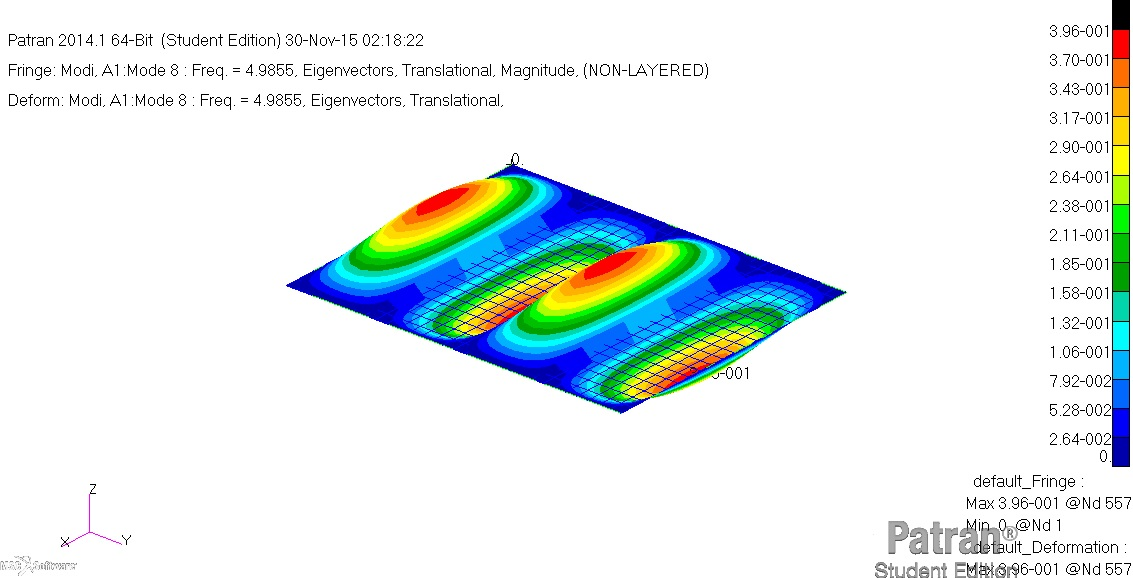
\includegraphics[width=.55\textwidth]{Immagini/modo8p.jpg}} \quad
	\subfloat[][\emph{Modo 8 Analitico}.]
	{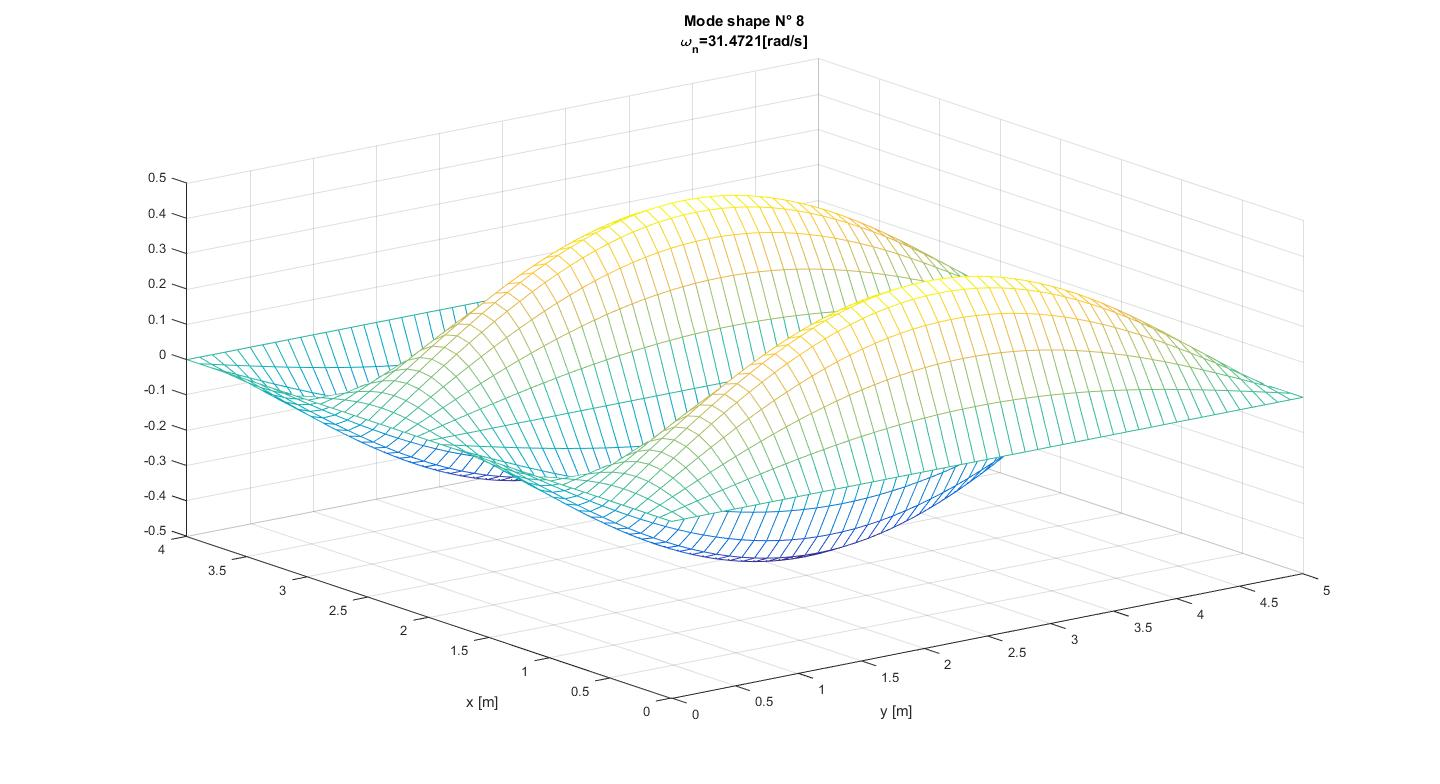
\includegraphics[width=.55\textwidth]{Immagini/modo8.jpg}} 
	\label{fig:subfig}
\end{figure}

\begin{figure}
	\subfloat[][\emph{Modo 9 FEM}.]
	{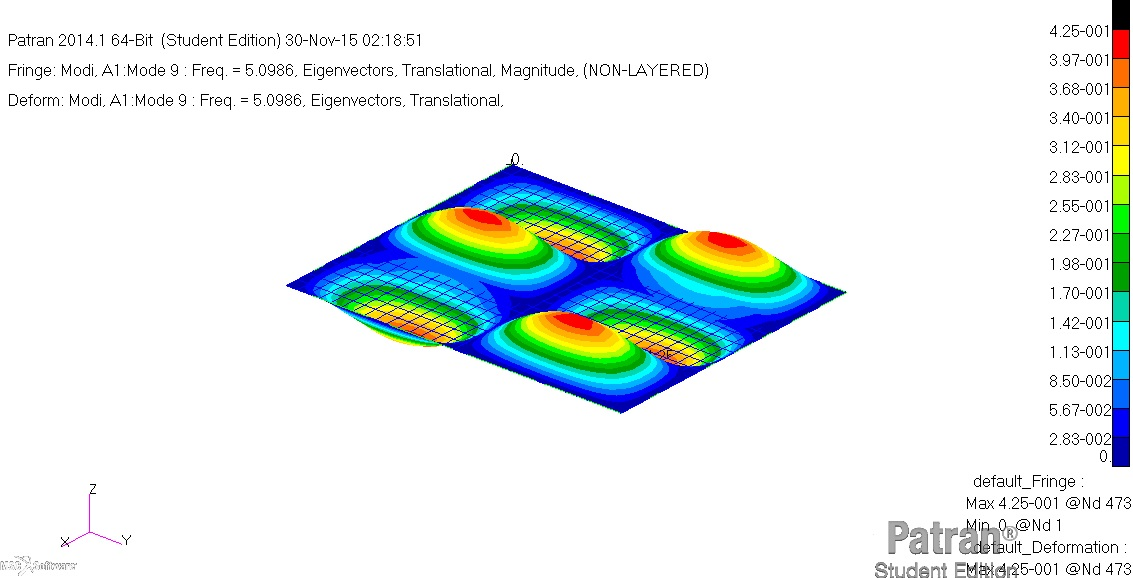
\includegraphics[width=.55\textwidth]{Immagini/modo9p.jpg}} \quad
	\subfloat[][\emph{Modo 9 Analitico}.]
	{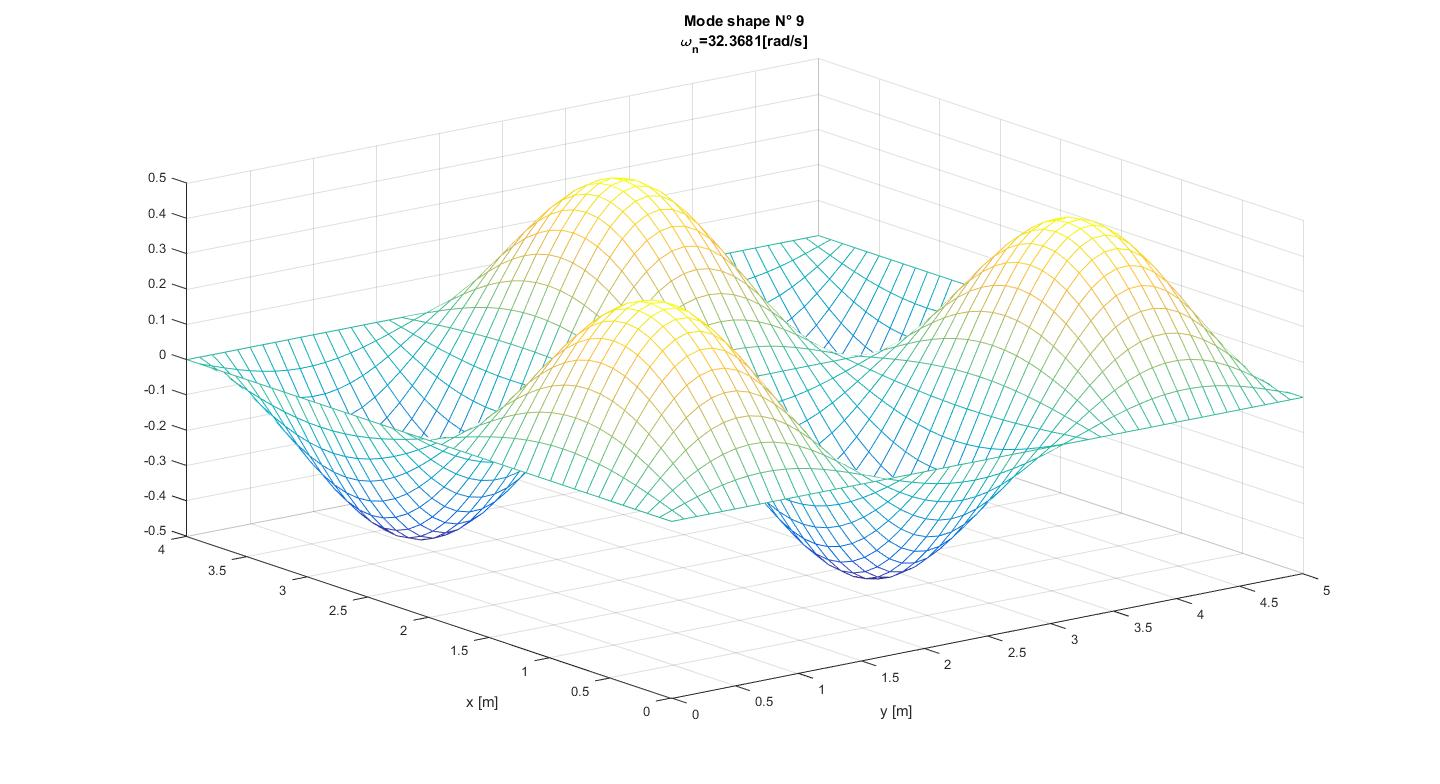
\includegraphics[width=.55\textwidth]{Immagini/modo9.jpg}} 
	\label{fig:subfig}
\end{figure}

\begin{figure}
	\subfloat[][\emph{Modo 10 FEM}.]
	{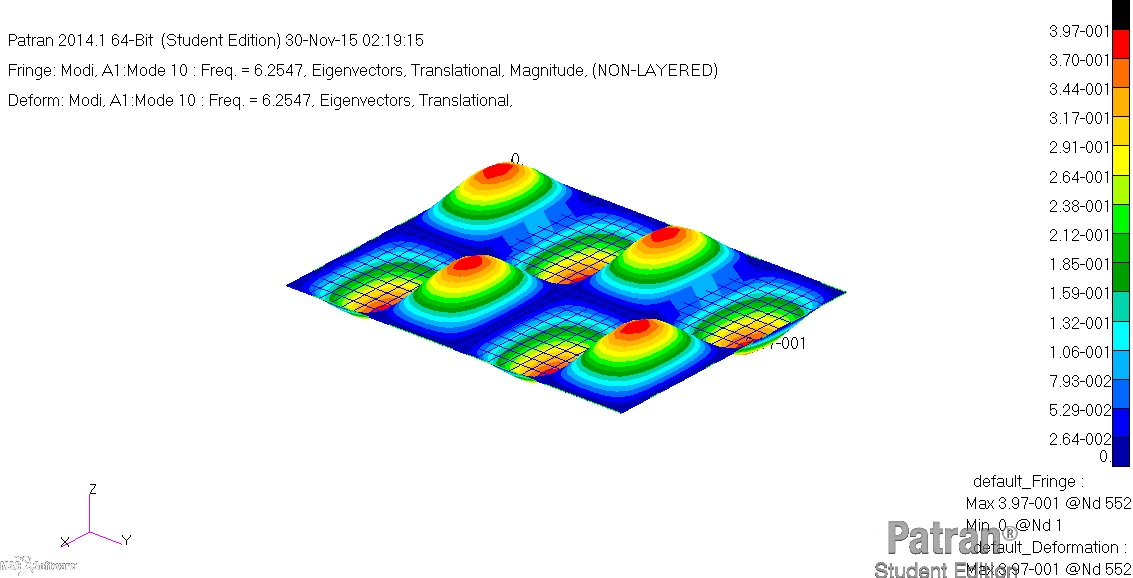
\includegraphics[width=.55\textwidth]{Immagini/modo10p.jpg}} \quad
	\subfloat[][\emph{Modo 10 Analitico}.]
	{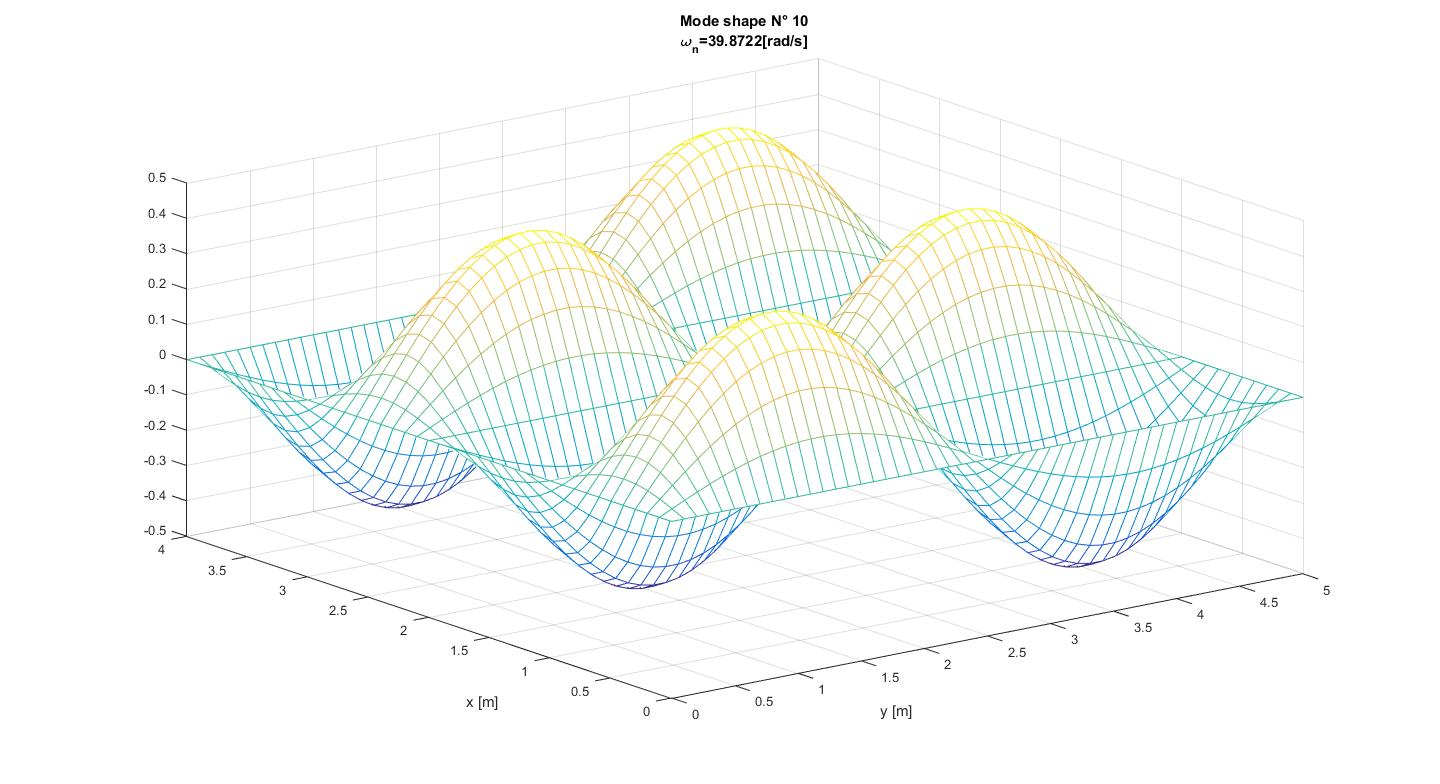
\includegraphics[width=.55\textwidth]{Immagini/modo10.jpg}} 
	\label{fig:subfig}
\end{figure}

\begin{figure}
	\subfloat[][\emph{Modo 11 FEM}.]
	{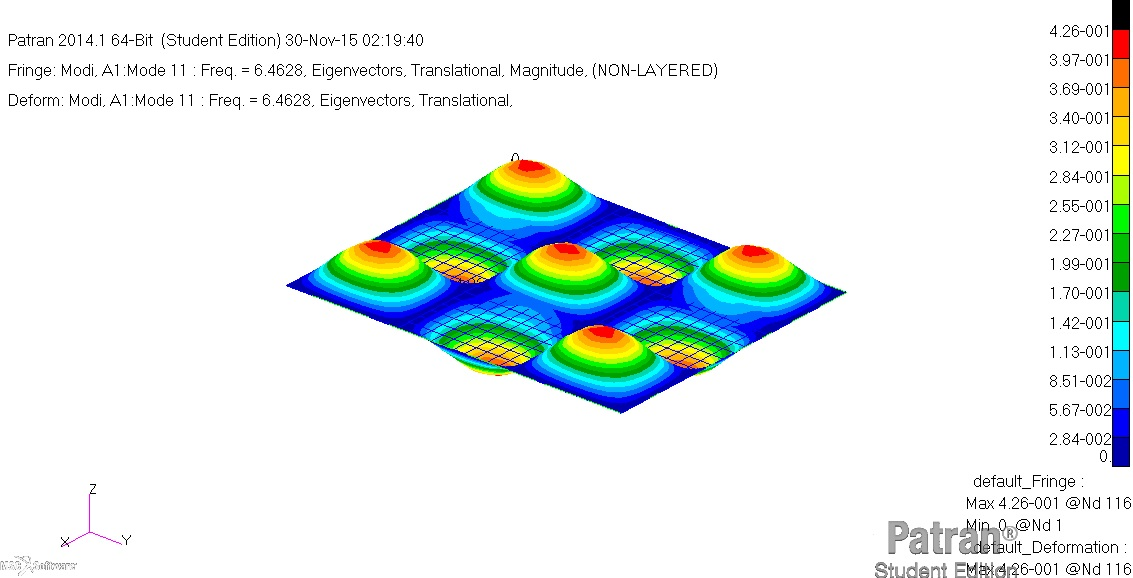
\includegraphics[width=.55\textwidth]{Immagini/modo11p.jpg}} \quad
	\subfloat[][\emph{Modo 11 Analitico}.]
	{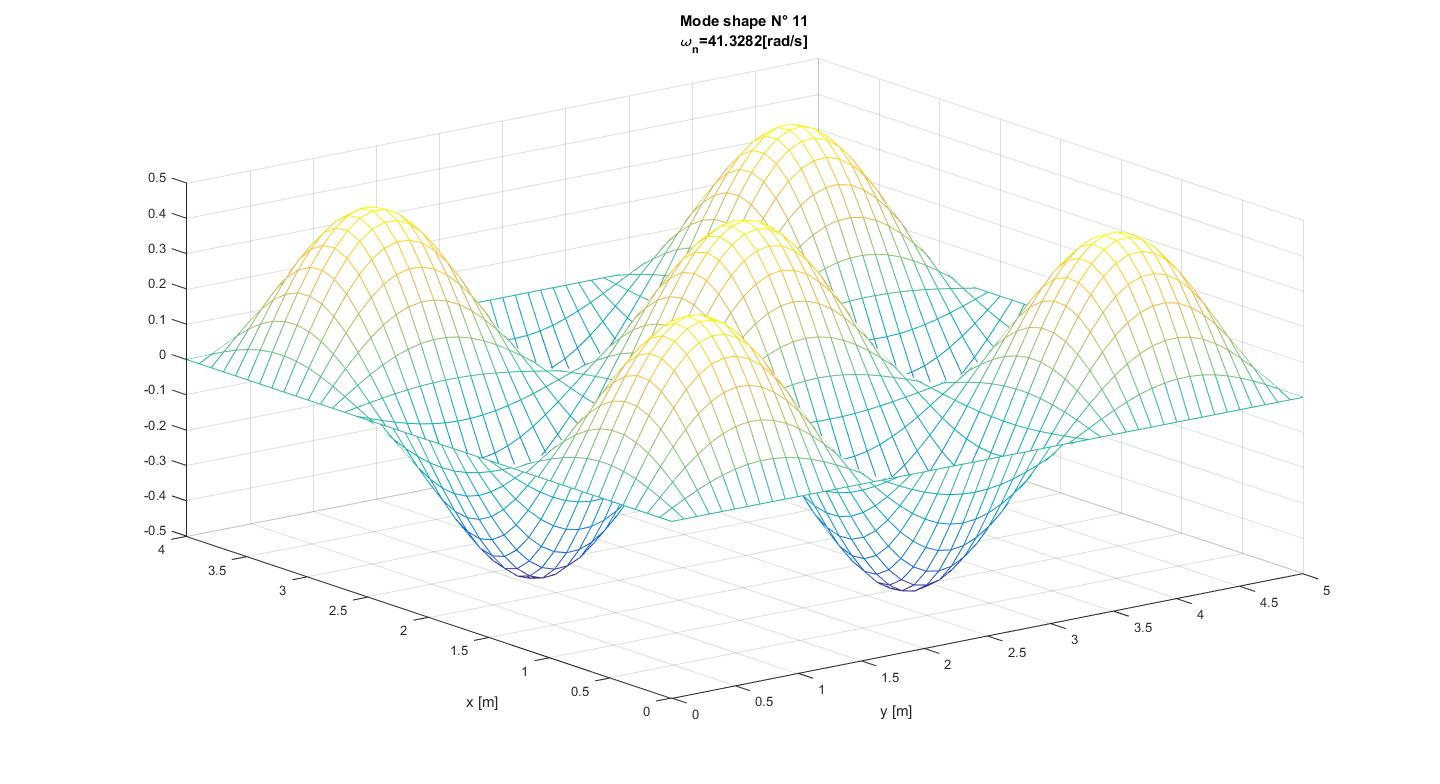
\includegraphics[width=.55\textwidth]{Immagini/modo11.jpg}} 
	\label{fig:subfig}
\end{figure}
\begin{figure}
	\subfloat[][\emph{Modo 12 FEM}.]
	{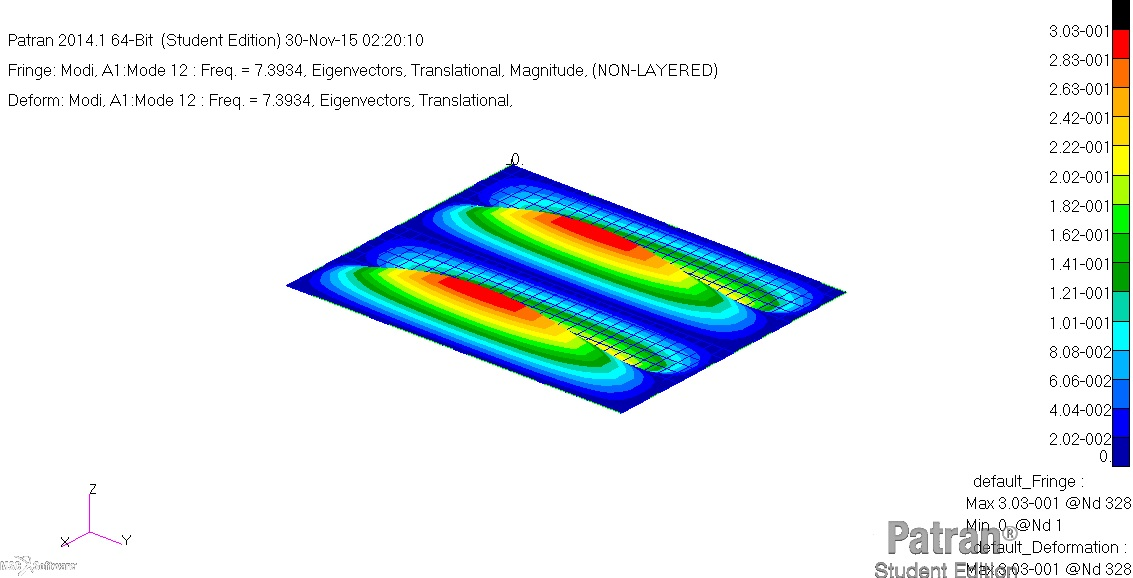
\includegraphics[width=.55\textwidth]{Immagini/modo12p.jpg}} \quad
	\subfloat[][\emph{Modo 12 Analitico}.]
	{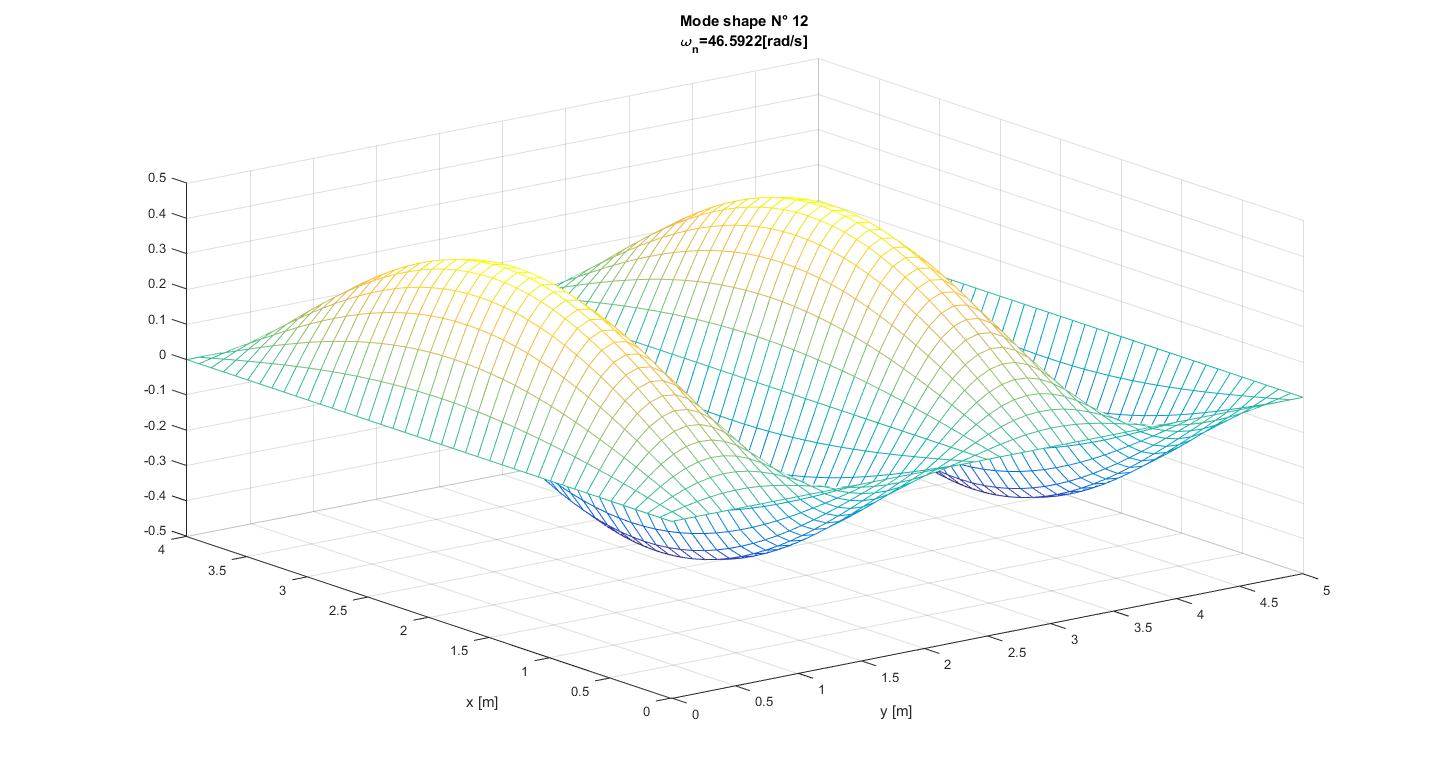
\includegraphics[width=.55\textwidth]{Immagini/modo12.jpg}} 
	\label{fig:subfig}
\end{figure}
\end{document}